\documentclass[]{article}
\usepackage{lmodern}
\usepackage{amssymb,amsmath}
\usepackage{ifxetex,ifluatex}
\usepackage{fixltx2e} % provides \textsubscript
\ifnum 0\ifxetex 1\fi\ifluatex 1\fi=0 % if pdftex
  \usepackage[T1]{fontenc}
  \usepackage[utf8]{inputenc}
\else % if luatex or xelatex
  \ifxetex
    \usepackage{mathspec}
    \usepackage{xltxtra,xunicode}
  \else
    \usepackage{fontspec}
  \fi
  \defaultfontfeatures{Mapping=tex-text,Scale=MatchLowercase}
  \newcommand{\euro}{€}
\fi
% use upquote if available, for straight quotes in verbatim environments
\IfFileExists{upquote.sty}{\usepackage{upquote}}{}
% use microtype if available
\IfFileExists{microtype.sty}{%
\usepackage{microtype}
\UseMicrotypeSet[protrusion]{basicmath} % disable protrusion for tt fonts
}{}
\usepackage[margin=1in]{geometry}
\usepackage{color}
\usepackage{fancyvrb}
\newcommand{\VerbBar}{|}
\newcommand{\VERB}{\Verb[commandchars=\\\{\}]}
\DefineVerbatimEnvironment{Highlighting}{Verbatim}{commandchars=\\\{\}}
% Add ',fontsize=\small' for more characters per line
\usepackage{framed}
\definecolor{shadecolor}{RGB}{248,248,248}
\newenvironment{Shaded}{\begin{snugshade}}{\end{snugshade}}
\newcommand{\KeywordTok}[1]{\textcolor[rgb]{0.13,0.29,0.53}{\textbf{{#1}}}}
\newcommand{\DataTypeTok}[1]{\textcolor[rgb]{0.13,0.29,0.53}{{#1}}}
\newcommand{\DecValTok}[1]{\textcolor[rgb]{0.00,0.00,0.81}{{#1}}}
\newcommand{\BaseNTok}[1]{\textcolor[rgb]{0.00,0.00,0.81}{{#1}}}
\newcommand{\FloatTok}[1]{\textcolor[rgb]{0.00,0.00,0.81}{{#1}}}
\newcommand{\CharTok}[1]{\textcolor[rgb]{0.31,0.60,0.02}{{#1}}}
\newcommand{\StringTok}[1]{\textcolor[rgb]{0.31,0.60,0.02}{{#1}}}
\newcommand{\CommentTok}[1]{\textcolor[rgb]{0.56,0.35,0.01}{\textit{{#1}}}}
\newcommand{\OtherTok}[1]{\textcolor[rgb]{0.56,0.35,0.01}{{#1}}}
\newcommand{\AlertTok}[1]{\textcolor[rgb]{0.94,0.16,0.16}{{#1}}}
\newcommand{\FunctionTok}[1]{\textcolor[rgb]{0.00,0.00,0.00}{{#1}}}
\newcommand{\RegionMarkerTok}[1]{{#1}}
\newcommand{\ErrorTok}[1]{\textbf{{#1}}}
\newcommand{\NormalTok}[1]{{#1}}
\ifxetex
  \usepackage[setpagesize=false, % page size defined by xetex
              unicode=false, % unicode breaks when used with xetex
              xetex]{hyperref}
\else
  \usepackage[unicode=true]{hyperref}
\fi
\hypersetup{breaklinks=true,
            bookmarks=true,
            pdfauthor={Carlos Espino García},
            pdftitle={Simulation Project},
            colorlinks=true,
            citecolor=blue,
            urlcolor=blue,
            linkcolor=magenta,
            pdfborder={0 0 0}}
\urlstyle{same}  % don't use monospace font for urls
\setlength{\parindent}{0pt}
\setlength{\parskip}{6pt plus 2pt minus 1pt}
\setlength{\emergencystretch}{3em}  % prevent overfull lines
\setcounter{secnumdepth}{5}

%%% Use protect on footnotes to avoid problems with footnotes in titles
\let\rmarkdownfootnote\footnote%
\def\footnote{\protect\rmarkdownfootnote}

%%% Change title format to be more compact
\usepackage{titling}
\setlength{\droptitle}{-2em}
  \title{Simulation Project}
  \pretitle{\vspace{\droptitle}\centering\huge}
  \posttitle{\par}
  \author{Carlos Espino García}
  \preauthor{\centering\large\emph}
  \postauthor{\par}
  \predate{\centering\large\emph}
  \postdate{\par}
  \date{July 21, 2015}




\begin{document}

\maketitle


\section{Overview}

This project presents an investigation of the exponential distribution
and a comparison with the Central Limit Theorem. To achieve this, we
sample the averages of 40 exponentials and analyze the distribution.
First, we campare the sample and theoretical mean of averages; second,
we campare the sample and theoretical variance of averages and at last
we verify the normality of the distribution.

\section{Simulations}

We generate a sample of size 1000 of the average of 40 exponentials. We
set \(\lambda = 0.2\) for all of the simulations.

\begin{Shaded}
\begin{Highlighting}[]
\NormalTok{lambda =}\StringTok{ }\FloatTok{0.2}
\KeywordTok{set.seed}\NormalTok{(}\DecValTok{15}\NormalTok{)}
\NormalTok{means =}\StringTok{ }\KeywordTok{unlist}\NormalTok{(}\KeywordTok{lapply}\NormalTok{(}\DecValTok{1}\NormalTok{:}\DecValTok{1000}\NormalTok{, function(x)\{}\KeywordTok{mean}\NormalTok{(}\KeywordTok{rexp}\NormalTok{(}\DecValTok{40}\NormalTok{, lambda))\}))}
\end{Highlighting}
\end{Shaded}

\section{Sample Mean versus Theoretical Mean}

The theoretical mean is given by: \[
\mbox{E}\left[\bar{X}\right] = \frac{1}{\lambda},
\]

which results in

\begin{Shaded}
\begin{Highlighting}[]
\NormalTok{theo_mean =}\StringTok{ }\NormalTok{(}\DecValTok{1}\NormalTok{/lambda)}
\NormalTok{theo_mean}
\end{Highlighting}
\end{Shaded}

\begin{verbatim}
## [1] 5
\end{verbatim}

We compute the sample mean

\begin{Shaded}
\begin{Highlighting}[]
\NormalTok{sample_mean =}\StringTok{ }\KeywordTok{mean}\NormalTok{(means)}
\NormalTok{sample_mean}
\end{Highlighting}
\end{Shaded}

\begin{verbatim}
## [1] 4.980535
\end{verbatim}

The relative difference is

\begin{Shaded}
\begin{Highlighting}[]
\NormalTok{(theo_mean-sample_mean)/theo_mean}
\end{Highlighting}
\end{Shaded}

\begin{verbatim}
## [1] 0.003892954
\end{verbatim}

\section{Sample Variance versus Theoretical Variance}

The theoretical variance is given by: \[
\mbox{Var}\left(\bar{X}\right) = \frac{1}{n\lambda},
\]

which results in

\begin{Shaded}
\begin{Highlighting}[]
\NormalTok{theo_var =}\StringTok{ }\NormalTok{(}\DecValTok{1}\NormalTok{/lambda^}\DecValTok{2}\NormalTok{)/}\DecValTok{40}
\NormalTok{theo_var}
\end{Highlighting}
\end{Shaded}

\begin{verbatim}
## [1] 0.625
\end{verbatim}

We compute the sample variance

\begin{Shaded}
\begin{Highlighting}[]
\NormalTok{sample_var =}\StringTok{ }\KeywordTok{var}\NormalTok{(means)}
\NormalTok{sample_var}
\end{Highlighting}
\end{Shaded}

\begin{verbatim}
## [1] 0.6186672
\end{verbatim}

The relative difference is

\begin{Shaded}
\begin{Highlighting}[]
\NormalTok{(theo_var-sample_var)/theo_var}
\end{Highlighting}
\end{Shaded}

\begin{verbatim}
## [1] 0.01013243
\end{verbatim}

\section{Distribution}

According to the Central Limit Theorem, the sample mean follows
asymptotically a normal distribution with the theoretical mean and
variance given in the previous sections.

To prove the normality, first we present a QQ-plot. As shown in Figure
\ref{fig:qqplot}, the points match the normal line, which means that the
quantiles of the sample approximately match with the quantiles of the
theoretical normal dstribution.

Then, Figure \ref{fig:histogram}, shows the histogram of the sample and
compares it with the bell of the normal density having the mean of the
sample mean of the averages and the sample variance of the averages. As
we can see, the histogram matches the bell curve, giving evidence of the
normality of the average.

At last, we provide a comparison between the distribution of a
collection of random exponentials and the distribution of a large
collection of averages of 40 exponentials. As Figure
\ref{fig:expcomparison} shows, the shape of the density of the averages
is like a normal density, which is coherent with the Central Limit
Theorem.

\begin{figure}

{\centering 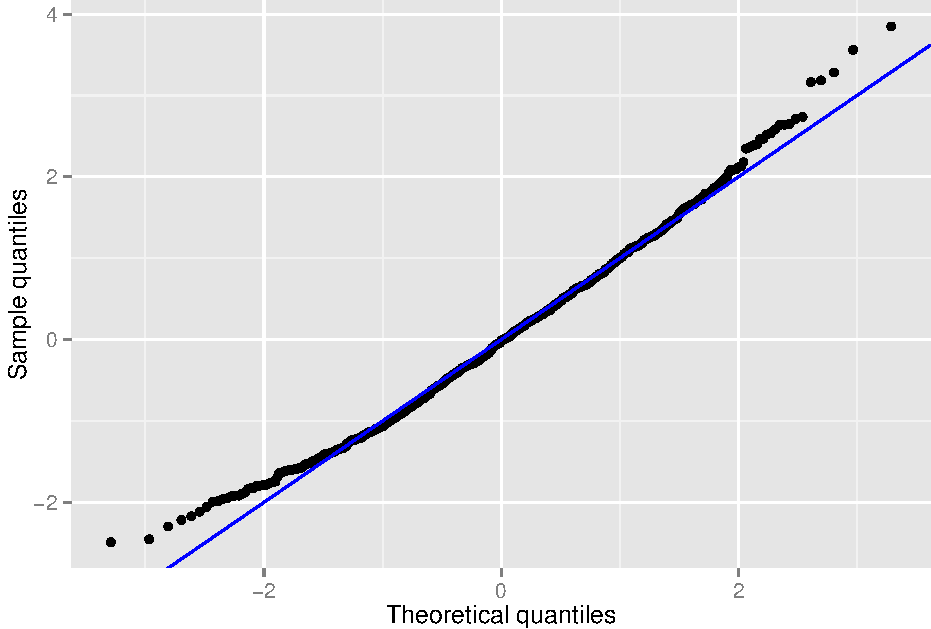
\includegraphics[width=.7\textwidth]{Simulation_Project_files/figure-latex/qqplot-1} 

}

\caption{QQ-plot Sample Quantiles Vs. Theoretical Quantiles}\label{fig:qqplot}
\end{figure}

\begin{figure}

{\centering 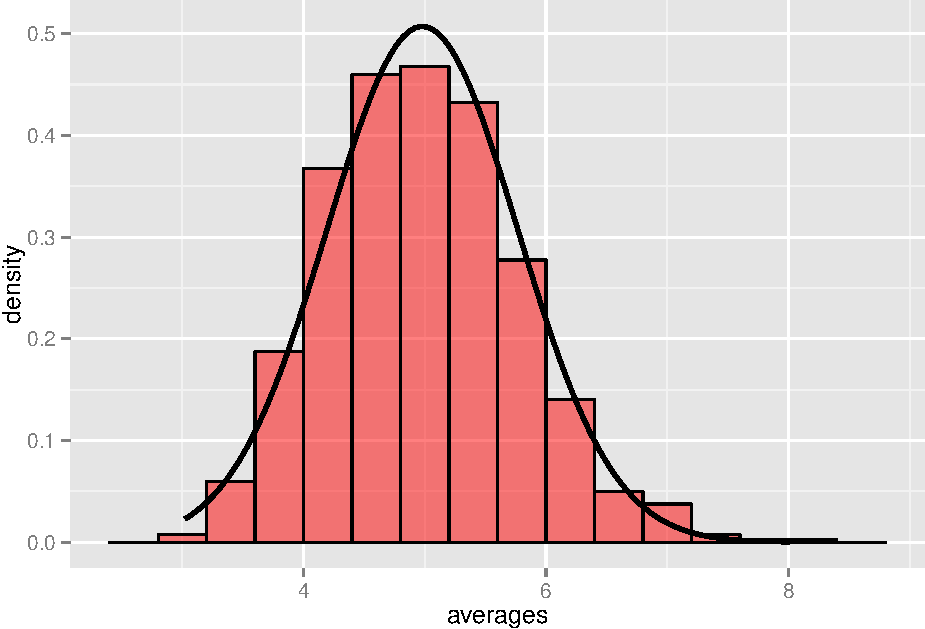
\includegraphics[width=.7\textwidth]{Simulation_Project_files/figure-latex/histogram-1} 

}

\caption{Histogram Vs. Theoretical normal density}\label{fig:histogram}
\end{figure}

\begin{figure}

{\centering 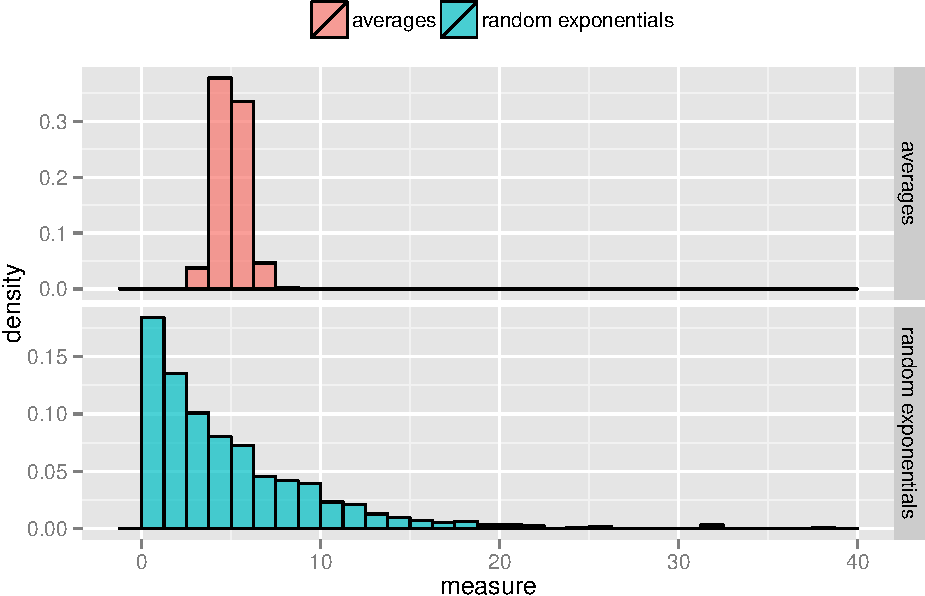
\includegraphics[width=.7\textwidth]{Simulation_Project_files/figure-latex/expcomparison-1} 

}

\caption{Averages sample Vs. Average of exponentials sample}\label{fig:expcomparison}
\end{figure}

\end{document}
